%-------------------------------------
% This template comes from Clara Eleonore Pavillet. 

% The Beamer Theme has been modified by Dr. Rahul Raoniar to fulfill B.Tech/Master/Ph.D./PostDoc student's Dissertation/Thesis/Proposal requirements.

% Description: I made this unofficial Beamer Template for the Indian Institute of Technology Bombay (IITB). Feel free to use it, modify it, and share it. 

% Thank you note: A huge thanks goes to Clara Eleonore Pavillet for the original template.
%-------------------------------------

\documentclass[aspectratio=169]{beamer}
\input{Theme/Packages.tex}
\usetheme{oxonian}
\usepackage{xcolor}
\usepackage{booktabs}
\usepackage{colortbl}
\usepackage{graphicx}
\definecolor{cmindsblue}{HTML}{1E4483}
% Footline colors
\setbeamercolor{footline}{fg=white,bg=cmindsblue}
\setbeamercolor{author in head/foot}{fg=white,bg=cmindsblue}
\setbeamercolor{title in head/foot}{fg=white,bg=cmindsblue}
\setbeamercolor{date in head/foot}{fg=white,bg=cmindsblue}
\setbeamercolor{structure}{fg=cmindsblue}
\setbeamercolor{frametitle}{fg=cmindsblue}

% Title page
\title{\textbf{\textcolor{purple}{Mirror Descent with Implicit Bias in Deep Learning}}}

% Sub-title
\subtitle{DS 608 Paper Presentation}

\titlegraphic{
\includegraphics[width=5cm]{Theme/Logos/cminds_iitb_logo.png}}

\author{\footnotesize \textbf{\textcolor{cmindsblue}{Chaitanya Deshkar}} \newline Under the Supervision of \newline \textbf{\textcolor{cmindsblue}{Pranay Sharma \vspace{4mm}}}}

\institute{\footnotesize \textbf{Indian Institute of Technology Bombay}\\ \vspace{1mm} Centre for Machine Intelligence and Data Science(C-MInDS)}

\date{\tiny April 06, 2026} %\today


\begin{document}

{\setbeamertemplate{footline}{} 
\frame{\titlepage}}

%%%%%%%%%%%%%%%%%%%%%%%%%%%%%%%%%%%%%%%%
% Outline
\section*{Outline}
\begin{frame}[fragile]
    {\textcolor{cmindsblue}{\textbf{Presentation Outline}}}
    \vspace{-0.2cm}
    {\tiny
    \tableofcontents[hideallsubsections, subsubsectionstyle=hide]
    }
\end{frame}

%%%%%%%%%%%%%%%%%%%%%%%%%%%%%%%%%%%%%%%%
% Section: Introduction 
%%%%%%%%%%%%%%%%%%%%%%%%%%%%%%%%%%%%%%%%
\section{\textbf{\textcolor{purple}{Introduction}}}
\begin{frame}[plain]
    \vfill
    \centering
    \begin{beamercolorbox}[sep=8pt,center,shadow=true,rounded=true]{title}
        \usebeamerfont{title}\insertsectionhead\par%
        \color{oxfordblue}\noindent\rule{10cm}{1pt}
    \end{beamercolorbox}
    \vfill
\end{frame}

%---------------------------------------
% Slide: The Deep Learning Boom
%---------------------------------------
\begin{frame}{\textcolor{cmindsblue}{\textbf{The Rise of Deep Learning}}}
    \vspace{-0.5cm}
    \begin{block}{\textbf{\textcolor{teal}{The 2012 Moment}}}
        \begin{itemize}
            \item AlexNet wins ImageNet 2012 by a ~10\% margin over second place — the moment the field took notice
        \end{itemize}
    \end{block}
    
    \begin{block}{\textbf{\textcolor{teal}{What Made It Work?}}}
        \begin{itemize}
            \item Massive overparameterization ($p \gg n$), SGD training, and empirical regularization techniques (dropout, batch norm)
        \end{itemize}
    \end{block}
    
    \vspace{0.2cm}
    \textit{But this raised a puzzle: classical learning theory predicted catastrophic overfitting.}
\end{frame}

%---------------------------------------
% Slide: Zhang et al. Experiment
%---------------------------------------
\begin{frame}{\textcolor{cmindsblue}{\textbf{The Generalization Mystery: Zhang et al. (2017)}}}
    \vspace{-0.3cm}
    \textbf{Same architecture, same optimizer, same hyperparameters. Only the labels changed:}
    \vspace{0.2cm}
    
    \begin{table}
    \centering
    \small
    \begin{tabular}{llcc}
    \toprule
    \textbf{Model} & \textbf{Condition} & \textbf{Train Acc.} & \textbf{Test Acc.} \\
    \midrule
    Inception & True labels        & 100\% & $\sim$87\% \\
    \rowcolor{orange!15}
    Inception & Random labels      & 100\% & $\sim$10\% \\
    \rowcolor{orange!15}
    Inception & Random pixels      & 100\% & $\sim$10\% \\
    \midrule
    AlexNet   & True labels        & 100\% & $\sim$80\% \\
    \rowcolor{orange!15}
    AlexNet   & Random labels      & 100\% & $\sim$10\% \\
    \midrule
    MLP       & True labels        & 100\% & $\sim$53\% \\
    \rowcolor{orange!15}
    MLP       & Random labels      & 100\% & $\sim$10\% \\
    \bottomrule
    \end{tabular}
    \caption*{\footnotesize CIFAR-10. Zhang et al., ICLR 2017.}
    \end{table}
    
    \vspace{0.1cm}
    \textbf{Model, size, optimizer, regularizer are identical across rows. Only labels differ. None of these explain generalization.}
\end{frame}

%---------------------------------------
% Slide: Classical Theory Fails
%---------------------------------------
\begin{frame}{\textcolor{cmindsblue}{\textbf{Classical Theory Cannot Explain This}}}
    \vspace{-0.3cm}
    \begin{block}{\textbf{\textcolor{teal}{Classical Generalization Bound}}}
    $$\text{Test error} \leq \text{Train error} + \underbrace{f(\text{model complexity}, n)}_{\text{complexity penalty}}$$
    \end{block}
    
    \begin{itemize}
        \item Since networks fit \textit{random} labels, their effective VC dimension / Rademacher complexity is essentially unbounded
        \item Therefore the complexity penalty is vacuously large — the bound predicts the network \textit{should not} generalize even on true labels
    \end{itemize}
    
    \begin{block}{\textbf{\textcolor{teal}{The Implication}}}
        Networks memorize noise yet generalize on real data. This contradiction vanishes if the optimizer itself creates the bias.
    \end{block}
\end{frame}

%---------------------------------------
% Slide: Implicit Bias Hypothesis
%---------------------------------------
\begin{frame}{\textcolor{cmindsblue}{\textbf{Implicit Bias: The Optimizer as Regularizer}}}
    \vspace{-0.3cm}
    \textbf{Setup:} In the overparameterized regime, the solution set $\mathcal{W}$ is a high-dimensional manifold — infinitely many zero-loss solutions exist.
    
    \begin{block}{\textbf{\textcolor{teal}{Known Result (Gunasekar et al., 2018)}}}
        For linear models, SGD converges to minimum $\ell_2$ norm interpolant by geometry, not explicit constraint.
    \end{block}
    
    \vspace{0.2cm}
    \textbf{Three open questions that this paper answers:}
    \begin{enumerate}
        \item What is the implicit bias for optimizers \textit{beyond} SGD?
        \item Does this extend to \textit{nonlinear} models like deep networks?
        \item Can we \textit{deliberately engineer} the implicit bias by choosing the optimizer?
    \end{enumerate}
    
    \vspace{0.2cm}
    \textit{If (3) is yes, the optimizer is a design choice for generalization.}
\end{frame}

%---------------------------------------
% Slide: Mirror Descent Framework
%---------------------------------------
\begin{frame}{\textcolor{cmindsblue}{\textbf{A Unified View: Stochastic Mirror Descent}}}
    \vspace{-0.3cm}
    \begin{block}{\textbf{\textcolor{teal}{SGD is just one special case}}}
        SMD generalizes all gradient-based optimizers via a potential function $\psi$
    \end{block}
    
    \vspace{0.2cm}
    \begin{table}
    \centering
    \small
    \begin{tabular}{lll}
    \hline
    \textbf{Potential $\psi(w)$} & \textbf{Algorithm} & \textbf{Implicit Bias} \\
    \hline
    $\frac{1}{2}\|w\|_2^2$ & SGD & Min $\ell_2$ norm \\
    $\sum_j w_j \log w_j$ & Exponentiated Gradient & Sparsity / simplex \\
    $\frac{1}{p}\|w\|_p^p$ & $p$-norm algorithm & Min $\ell_p$ norm \\
    \hline
    \end{tabular}
    \end{table}
    
    \vspace{0.2cm}
    \textbf{The choice of $\psi$ is the choice of bias. This paper proves which solution SMD finds for any $\psi$ in nonlinear models.}
\end{frame}

%%%%%%%%%%%%%%%%%%%%%%%%%%%%%%%%%%%%%%%%
% Section: Problem Setup
%%%%%%%%%%%%%%%%%%%%%%%%%%%%%%%%%%%%%%%%
\section{\textbf{\textcolor{purple}{Problem Setup and Notation}}}
\begin{frame}[plain]
    \vfill
    \centering
    \begin{beamercolorbox}[sep=8pt,center,shadow=true,rounded=true]{title}
        \usebeamerfont{title}\insertsectionhead\par%
        \color{oxfordblue}\noindent\rule{10cm}{1pt}
    \end{beamercolorbox}
    \vfill
\end{frame}

%---------------------------------------
% Slide: Mathematical Framework
%---------------------------------------
\begin{frame}{\textcolor{cmindsblue}{\textbf{Overparameterized Nonlinear Models}}}
    \begin{itemize}
        \item \textbf{Dataset:} $\{(x_i, y_i)\}_{i=1}^n$ where $x_i \in \mathbb{R}^d$ and $y_i \in \mathbb{R}$.
        \item \textbf{Model:} $f(x_i, w) = f_i(w)$ with parameters $w \in \mathbb{R}^p$.
        \item \textbf{The Interpolating Regime:} $p \gg n$.
    \end{itemize}

    \begin{block}{The Set of Global Minima (Interpolants)}
        The set of all parameters consistent with the training data:
        \begin{equation}
            \mathcal{W} = \{w \in \mathbb{R}^p \mid f_i(w) = y_i, \quad i=1, \dots, n\}
        \end{equation}
        This forms a high-dimensional $(p-n)$-dimensional manifold.
    \end{block}

    \begin{block}{The Learning Objective}
        Minimize empirical risk $L(w) = \sum_{i=1}^n L_i(w)$, where $L_i(w) = \ell(y_i, f_i(w))$. Every $w \in \mathcal{W}$ yields $L(w) = 0$.
    \end{block}
\end{frame}

%---------------------------------------
% Slide: Stochastic Gradient Descent
%---------------------------------------
\begin{frame}{\textcolor{cmindsblue}{\textbf{Optimization via SGD}}}
    Standard training typically utilizes \textbf{Stochastic Gradient Descent (SGD)}:
    \begin{equation}
        w_i = w_{i-1} - \eta \nabla L_i(w_{i-1}), \quad i \geq 1
    \end{equation}
    
    \vspace{0.3cm}
    \begin{itemize}
        \item $L_i(\cdot)$ is differentiable and non-negative.
        \item $L_i(w) = 0$ iff $y_i = f_i(w)$.
        \item For $i > n$, we cycle through the data or select at random.
    \end{itemize}
    \vfill
    \begin{block}{\textbf{\textcolor{teal}{The Implicit Question}}}
    Among all $w \in \mathcal{W}$, SGD will converge to exactly one. The update rule's geometry — not any explicit constraint — determines which one. This is the implicit bias.
    \end{block}
\end{frame}

%%%%%%%%%%%%%%%%%%%%%%%%%%%%%%%%%%%%%%%%
% Section: Stochastic Mirror Descent
%%%%%%%%%%%%%%%%%%%%%%%%%%%%%%%%%%%%%%%%
\section{\textbf{\textcolor{purple}{Stochastic Mirror Descent (SMD)}}}
\begin{frame}[plain]
    \vfill
    \centering
    \begin{beamercolorbox}[sep=8pt,center,shadow=true,rounded=true]{title}
        \usebeamerfont{title}\insertsectionhead\par%
        \color{oxfordblue}\noindent\rule{10cm}{1pt}
    \end{beamercolorbox}
    \vfill
\end{frame}

%---------------------------------------
% Slide: Defining the Mirror Update
%---------------------------------------
\begin{frame}{\textcolor{cmindsblue}{\textbf{The Geometry of Mirror Descent}}}
    Instead of updating in the weight space, SMD updates in the \textbf{mirrored domain} via a strictly convex potential function $\psi(\cdot)$.
    
    \begin{block}{The Update Rule}
        \begin{equation}
            \nabla\psi(w_i) = \nabla\psi(w_{i-1}) - \eta\nabla L_i(w_{i-1})
        \end{equation}
    \end{block}

    \begin{itemize}
        \item Updates happen in dual space via $\nabla\psi$
        \item SGD: $\psi(w) = \frac{1}{2}\|w\|^2$ gives $\nabla\psi = \text{identity}$
        \item Different $\psi$ encode different geometric biases
    \end{itemize}
    
    \vspace{0.2cm}
    \textit{Every optimizer is mirror descent in disguise.}
\end{frame}

%---------------------------------------
% Slide: Bregman Divergence
%---------------------------------------
\begin{frame}{\textcolor{cmindsblue}{\textbf{The Bregman Perspective}}}
    The SMD update can be equivalently viewed as a proximal minimization problem:
    \begin{equation}
        w_i = \arg\min_{w} \left\{ \eta w^T \nabla L_i(w_{i-1}) + D_\psi(w, w_{i-1}) \right\}
    \end{equation}

    \begin{block}{Bregman Divergence $D_\psi(w, \bar{w})$}
        Defined as the difference between the function and its first-order Taylor expansion:
        \begin{equation}
            D_\psi(w, \bar{w}) := \psi(w) - \psi(\bar{w}) - \nabla\psi(\bar{w})^T(w - \bar{w})
        \end{equation}
    \end{block}

    \begin{itemize}
        \item Non-negative: $D_\psi(w, \bar{w}) \geq 0$, equals 0 iff $w = \bar{w}$
        \item Tailored to geometry of $\psi$
    \end{itemize}
\end{frame}

%---------------------------------------
% Slide: Implicit Bias in Linear Models
%---------------------------------------
\section{\textbf{\textcolor{purple}{Implicit Bias: The Linear Case}}}
\begin{frame}{\textcolor{cmindsblue}{\textbf{Implicit Regularization in Linear Models}}}
    Consider the overparameterized linear model $f(x_i, w) = x_i^T w$.
    
    \begin{block}{Proposition 1: Convergence to the Closest Interpolant}
        For a sufficiently small step size $\eta$, the SMD iterates converge to:
        \begin{equation}
            w_\infty = \arg\min_{w \in \mathcal{W}} D_\psi(w, w_0)
        \end{equation}
    \end{block}

    \begin{itemize}
        \item Out of infinite $\mathcal{W}$ solutions, SMD picks the Bregman-closest to initialization
        \item If $w_0 = \arg\min_w \psi(w)$, then $w_\infty = \arg\min_{w \in \mathcal{W}} \psi(w)$
        \item Geometry is the regularizer
    \end{itemize}
    
    \begin{block}{\textbf{\textcolor{teal}{Implication}}}
    First rigorous answer to Zhang et al.: optimizer encodes preference. This is determined by $\psi$ and $w_0$.
    \end{block}
\end{frame}

%%%%%%%%%%%%%%%%%%%%%%%%%%%%%%%%%%%%%%%%
% Section: Assumptions and Theorems
%%%%%%%%%%%%%%%%%%%%%%%%%%%%%%%%%%%%%%%%
\section{\textbf{\textcolor{purple}{Nonlinear Analysis: Assumptions and Main Results}}}

\subsection{\textbf{\textcolor{purple}{Key Assumptions}}}
\begin{frame}[plain]
    \vfill
    \centering
    \begin{beamercolorbox}[sep=8pt,center,shadow=true,rounded=true]{title}
        \usebeamerfont{title}Assumptions for Nonlinear Models\par%
        \color{oxfordblue}\noindent\rule{10cm}{1pt}
    \end{beamercolorbox}
    \vfill
\end{frame}

%---------------------------------------
% Slide: Theoretical Assumptions
%---------------------------------------


\begin{frame}{Assumption 1: Local Star-Convexity}
    \vspace{-0.3cm}
    \textbf{Setup:} Define region $\mathcal{B} = \{w \in \mathbb{R}^p \mid D_\psi(w, \bar{w}) \leq \epsilon\}$ containing $w_0$.\vspace{0.15cm}
    
    \textbf{Assumption Statement:} There exists $\bar{w} \in \mathcal{W}$ such that
    $$D_{L_i}(\bar{w}, w) := L_i(\bar{w}) - L_i(w) - \nabla L_i(w)^T(\bar{w} - w) \geq 0$$
    \vspace{0.15cm}
    for all $w \in \mathcal{B}$ and $i = 1, \ldots, n$.
    
    \textbf{Geometric interpretation:} The loss Bregman divergence is non-negative. This means the region near interpolating solutions exhibits local "star-convexity": curvature points inward toward the solution set.
    
    \textbf{Why it's reasonable:} In the overparameterized regime ($p \gg n$), near any solution $\bar{w} \in \mathcal{W}$, the effective loss landscape becomes benign due to the abundance of degrees of freedom.
\end{frame}

\begin{frame}{Assumption 2: Boundedness}
    Model $f_i(w)$ has bounded derivatives in $\mathcal{B}$. \vspace{0.2cm}
    
    \begin{itemize}
        \item Gradient: $\|\nabla f_i(w)\| \leq \gamma$
        \item Hessian: $\alpha I \preceq H_{f_i}(w) \preceq \beta I$ for constants $\alpha, \beta$
    \end{itemize}
    
    These prevent divergence under fixed step size $\eta$.
\end{frame}

%%%%%%%%%%%%%%%%%%%%%%%%%%%%%%%%%%%%%%%%
% Section: Main Theorems
%%%%%%%%%%%%%%%%%%%%%%%%%%%%%%%%%%%%%%%%

\subsection{\textbf{\textcolor{purple}{Main Convergence and Characterization Results}}}
\begin{frame}[plain]
    \vfill
    \centering
    \begin{beamercolorbox}[sep=8pt,center,shadow=true,rounded=true]{title}
        \usebeamerfont{title}Main Theorems\par%
        \color{oxfordblue}\noindent\rule{10cm}{1pt}
    \end{beamercolorbox}
    \vfill
\end{frame}

\begin{frame}{Theorem 3: Deterministic Convergence}
    Under Assumption 1, and for a step size $\eta$ such that $\psi(\cdot) - \eta L_i(\cdot)$ is strictly convex for all $i$, the following hold for the SMD iterates $\{w_i\}$:
    
    \begin{enumerate}
        \item \textbf{Containment:} All iterates $\{w_i\}$ remain within the region $\mathcal{B}$.
        \item \textbf{Global Convergence:} The sequence $\{w_i\}$ converges to a limit $w_\infty$.
        \item \textbf{Interpolation:} The limit point is a global minimum, i.e., $w_\infty \in \mathcal{W}$.
    \end{enumerate}
    \vspace{0.3cm}
    \textbf{Note:} Deterministic convergence, no high-probability bounds needed.
    
    \vspace{0.2cm}
    \textbf{Key point:} Bregman geometry guarantees convergence independent of model.
\end{frame}

\begin{frame}{Theorem 4: Characterization of the Limit Point}
    Let $w^* = \arg\min_{w \in \mathcal{W}} D_\psi(w, w_0)$ be the Bregman-closest interpolant to the initialization.
    
    \begin{block}{Proximity to the Optimal Regularized Solution}
        Under Assumptions 1 and 2, the limit point $w_\infty$ satisfies:
        \begin{enumerate}
            \item $D_\psi(w_\infty, w_0) = D_\psi(w^*, w_0) + o(\epsilon)$
            \item $D_\psi(w^*, w_\infty) = o(\epsilon)$
        \end{enumerate}
    \end{block}
    \vspace{0.2cm}
    If $w_0$ is $O(\epsilon)$ from $\mathcal{W}$, then $w_\infty$ is $o(\epsilon)$ from $w^*$.
    
    \textbf{Result:} SMD implicitly minimizes $\psi$ over interpolants.
\end{frame}


%%%%%%%%%%%%%%%%%%%%%%%%%%%%%%%%%%%%%%%%
% Section: Proof Technique
%%%%%%%%%%%%%%%%%%%%%%%%%%%%%%%%%%%%%%%%
\section{\textbf{\textcolor{purple}{Proofs: Bregman Distance Analysis}}}

\subsection{\textbf{\textcolor{purple}{Fundamental Identity and Proof Technique}}}
\begin{frame}[plain]
    \vfill
    \centering
    \begin{beamercolorbox}[sep=8pt,center,shadow=true,rounded=true]{title}
        \usebeamerfont{title}Proof Technique: Fundamental Identity\par%
        \color{oxfordblue}\noindent\rule{10cm}{1pt}
    \end{beamercolorbox}
    \vfill
\end{frame}

\begin{frame}{Lemma 6: A General Identity for SMD}
    The authors derive a fundamental identity that holds for any model $f(\cdot, \cdot)$ and differentiable loss $\ell(\cdot)$. For any $w \in \mathcal{W}$:
    
    \begin{equation}
        D_\psi(w, w_{i-1}) = D_\psi(w, w_i) + D_{\psi - \eta L_i}(w_i, w_{i-1}) + \eta L_i(w_i) + \eta D_{L_i}(w, w_{i-1})
    \end{equation}
    
    \textbf{Algebraic structure:} All three RHS terms are non-negative (by convexity, non-negativity of loss, and star-convexity). This creates a telescoping inequality.
    
    \vspace{0.1cm}
    \textbf{Takeaway:} The Bregman distance to any interpolant is non-increasing, with three dissipative mechanisms:
    \begin{enumerate}
        \item Mirror-adjusted divergence shrapes solutions together
        \item Loss terms vanish as iterates converge
        \item Bregman loss divergence measures local geometry
    \end{enumerate}
\end{frame}

\begin{frame}{Lemma 6: Proof Derivation}
    \vspace{-0.25cm}
    Start with Bregman definition: $D_\psi(w, w_i) = \psi(w) - \psi(w_i) - \nabla\psi(w_i)^T(w - w_i)$.
    
    \vspace{0.08cm}
    Substitute SMD update: $\nabla\psi(w_i) = \nabla\psi(w_{i-1}) - \eta\nabla L_i(w_{i-1})$:
    $$D_\psi(w, w_i) = \psi(w) - \psi(w_i) - [\nabla\psi(w_{i-1}) - \eta\nabla L_i(w_{i-1})]^T(w-w_i)$$
    
    \vspace{0.08cm}
    Decompose by adding and subtracting $\psi(w_{i-1}) + \nabla\psi(w_{i-1})^T(w-w_{i-1})$:
    $$D_\psi(w,w_i) = [D_\psi(w,w_{i-1}) - D_\psi(w_i,w_{i-1})] + \eta\nabla L_i(w_{i-1})^T(w-w_i)$$
    
    \vspace{0.08cm}
    Expand $(w-w_i)=(w-w_{i-1})-(w_i-w_{i-1})$ and apply loss Bregman definitions.
    
    \vspace{0.08cm}
    \textbf{Result:} The fundamental identity with telescoping terms.
\end{frame}

\begin{frame}{Lemma 6: Full Mathematical Derivation (Detailed)}
    \vspace{-0.25cm}
    \textbf{Step 1.} Expand $D_\psi(w,w_i)$ and $D_\psi(w_i,w_{i-1})$ separately, then combine:
    \begin{align}
    D_\psi(w,w_i) &= D_\psi(w,w_{i-1}) - D_\psi(w_i,w_{i-1}) + \eta\nabla L_i(w_{i-1})^T(w-w_i)
    \end{align}
    
    \vspace{0.08cm}
    \textbf{Step 2.} For $w \in \mathcal{W}$, use $L_i(w) = 0$:
    $$\eta\nabla L_i(w_{i-1})^T(w-w_{i-1}) = \eta L_i(w) - \eta L_i(w_{i-1}) - \eta D_{L_i}(w,w_{i-1})$$
    (By definition of Bregman divergence for the loss.)
    
    \vspace{0.08cm}
    \textbf{Step 3.} Rearrange using $(w-w_i) = (w-w_{i-1})-(w_i-w_{i-1})$:
    $$\eta\nabla L_i(w_{i-1})^T(w-w_i) = -[L_i(w_{i-1})-L_i(w_i)-\nabla L_i(w_{i-1})^T(w_i-w_{i-1})] - \eta D_{L_i}(w,w_{i-1})$$
    $$= -D_{\psi-\eta L_i}(w_i,w_{i-1}) - \eta L_i(w_i) - \eta D_{L_i}(w,w_{i-1})$$
    
    \vspace{0.08cm}
    After rearrangement: the identity follows.
\end{frame}

\begin{frame}{Proof of Theorem 3: Containment and Convergence}
    \vspace{-0.25cm}
    \textbf{Part 1. Containment in $\mathcal{B}$:} From Lemma 6 (Fundamental Identity):
    $$D_\psi(w, w_{i-1}) = D_\psi(w, w_i) + D_{\psi - \eta L_i}(w_i, w_{i-1}) + \eta L_i(w_i) + \eta D_{L_i}(w, w_{i-1})$$
    
    For $w \in \mathcal{W}$: all RHS terms are non-negative (by strict convexity of $\psi - \eta L_i$, sign of loss, star-convexity assumption). Thus $D_\psi(w, w_i) \leq D_\psi(w, w_{i-1}) \leq \cdots \leq D_\psi(w, w_0) \leq \epsilon$. Iterates stay in $\mathcal{B}$.
    
    \vspace{0.08cm}
    \textbf{Part 2. Convergence:} Telescope Lemma 6 over $i=1,\ldots, T$. Boundary terms cancel:
    $$D_\psi(w,w_0) = D_\psi(w,w_T) + \sum_{i=1}^T [\text{non-negative terms}]$$
    
    Since $D_\psi(w,w_T) \geq 0$ and LHS is fixed, the sum is bounded: $T \to \infty$ forces each term to 0. In particular, $D_{\psi-\eta L_i}(w_i,w_{i-1}) \to 0$, so $w_i \to w_\infty$ (convergence).
    
    \vspace{0.08cm}
    \textbf{Part 3. Interpolation:} Loss terms $\eta L_i(w_i) \to 0$, so $L_i(w_\infty) = 0$ for all $i$. Thus $w_\infty \in \mathcal{W}$.
\end{frame}

\begin{frame}{Proof of Theorem 4: Closeness to Optimal Point}
    \vspace{-0.25cm}
    \textbf{Setup:} Apply Lemma 6 to both $w^*$ and $w_\infty$, both in $\mathcal{W}$. Telescope over all iterations:
    $$D_\psi(w^*,w_0) = D_\psi(w^*,w_\infty) + \sum_{i=1}^\infty [\cdots]$$
    $$D_\psi(w_\infty,w_0) = D_\psi(w_\infty,w_\infty) + \sum_{i=1}^\infty [\cdots] = \sum_{i=1}^\infty [\cdots]$$
    
    \vspace{0.08cm}
    \textbf{Key observation:} The sums depend on $w^*$ and $w_\infty$ only through their distance from intermediate iterates $w_{i-1}$. By Assumption 2 (bounded Hessian), these distances are $O(\epsilon)$.
    
    \vspace{0.08cm}
    \textbf{Conclusion:} Subtracting the two equations and using Hessian bounds via Taylor expansion:
    $$D_\psi(w_\infty,w_0) - D_\psi(w^*,w_0) = -D_\psi(w^*,w_\infty) + o(\epsilon)$$
    
    Since both $D_\psi(w_\infty,w_0) - D_\psi(w^*,w_0) \geq 0$ (by definition of $w^*$) and $D_\psi(w^*,w_\infty) \geq 0$, each is $o(\epsilon)$.
\end{frame}

\begin{frame}{Highly Overparameterized Regime: Why $w_0$ Is Close to $\mathcal{W}$}
    \vspace{-0.3cm}
    In the limit $p \gg n$, a random initialization is whp close to the interpolating set.
    
    \begin{block}{Linear Approximation Argument}
        \begin{itemize}
            \item Distance to $\mathcal{W}$ is approximated by the solution to the linearized problem:
            \begin{equation}
                \min_w \|w - w_0\|^2 \quad \text{s.t.} \quad y \approx f(x, w_0) + \nabla f(x, w_0)^T(w - w_0)
            \end{equation}
            \item The Jacobian $\nabla f(x, w_0)$ is $n \times p$, consisting of sums of outer products
        \end{itemize}
    \end{block}
    
    \begin{itemize}
        \item When $p \gg n$ and data are sufficiently random: $\lambda_{\min}(\nabla f^T \nabla f) = \Omega(p)$
        \item Thus: $\|w^* - w_0\|^2 \approx \|y - f(x, w_0)\|^2 \cdot O(1/p) = O(n/p)$
        \item Conclusion: $w_0$ is $O(\sqrt{n/p})$ away from the manifold—negligible as $p$ grows
    \end{itemize}
\end{frame}

%%%%%%%%%%%%%%%%%%%%%%%%%%%%%%%%%%%%%%%%
% Section: Experiments
%%%%%%%%%%%%%%%%%%%%%%%%%%%%%%%%%%%%%%%%
\section{\textbf{\textcolor{purple}{Experimental Validation}}}

\subsection{\textbf{\textcolor{purple}{Setup, Results, and Insights}}}
\begin{frame}[plain]
    \vfill
    \centering
    \begin{beamercolorbox}[sep=8pt,center,shadow=true,rounded=true]{title}
        \usebeamerfont{title}Experimental Validation\par%
        \color{oxfordblue}\noindent\rule{10cm}{1pt}
    \end{beamercolorbox}
    \vfill
\end{frame}

\begin{frame}{Experimental Setup}
    \vspace{-0.2cm}
    \textbf{Datasets:} MNIST (60K samples), CIFAR-10 (50K samples). Both highly overparameterized.
    
    \vspace{0.08cm}
    \textbf{Architectures:} MNIST: 4-layer CNN with 2M parameters. CIFAR-10: ResNet-18 with 11M parameters.
    
    \vspace{0.08cm}
    \textbf{Protocol:} Random initialization $\mathcal{N}(0, 0.0001)$, train to $100\%$ accuracy.
    
    \vspace{0.08cm}
    \textbf{Seeds:} 6 initializations (MNIST), 8 initializations (CIFAR-10).
    
    \vspace{0.08cm}
    \textbf{Algorithms:} Mirror potentials $\psi(w) = \frac{1}{q}\|w\|_q^q$ for $q \in \{1+\epsilon, 2, 3, 10\}$.
\end{frame}

\begin{frame}{Experimental Hypothesis}
    The paper predicts that \textbf{each SMD algorithm finds the interpolant closest to its initialization in the corresponding Bregman divergence}.
    
    \begin{block}{Testing Strategy}
        For each initialization $w_0$ and each mirror type (with potential $\psi$):
        \begin{enumerate}
            \item Train the model to zero training error, reaching some $w_\infty \in \mathcal{W}$
            \item Compute Bregman divergences $D_{\psi_q}(w_\infty^{(q)}, w_0)$ for all mirrors $q \in \{1+\epsilon, 2, 3, 10\}$
            \item Check: Is the minimum always on the diagonal?
        \end{enumerate}
    \end{block}
    
    \begin{itemize}
        \item \textbf{Prediction:} For fixed $w_0$ and fixed $\psi_q$, the closest final point to $w_0$ (in $D_{\psi_q}$ distance) should be the one obtained by running SMD with $\psi_q$
        \item This would confirm both convergence to $w^*$ and the theoretical characterization
    \end{itemize}
\end{frame}

\begin{frame}{MNIST Results: Convergence to Nearest Interpolant}
    \vspace{-0.25cm}
    \centering
    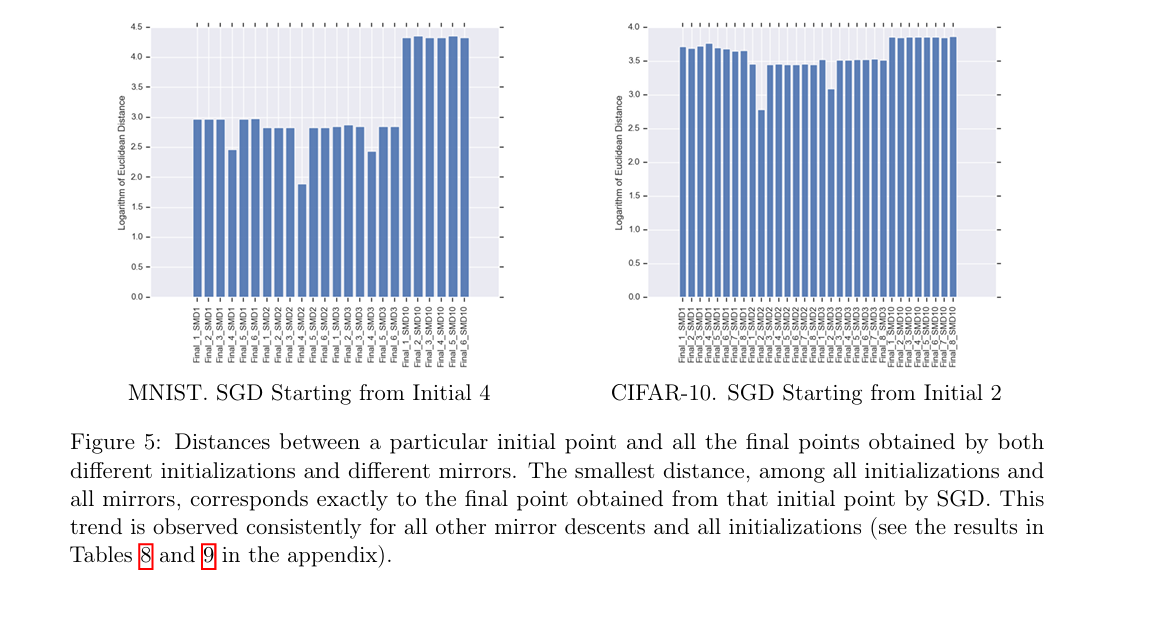
\includegraphics[width=0.95\textwidth]{images/L1vsL10.png}
    
    \vspace{-0.15cm}
    {\small Diagonal dominance: Each mirror finds its closest interpolant. Confirms Theorem 4.}
\end{frame}

\begin{frame}{CIFAR-10 Results: Consistency at Scale}
    \vspace{-0.25cm}
    \centering
    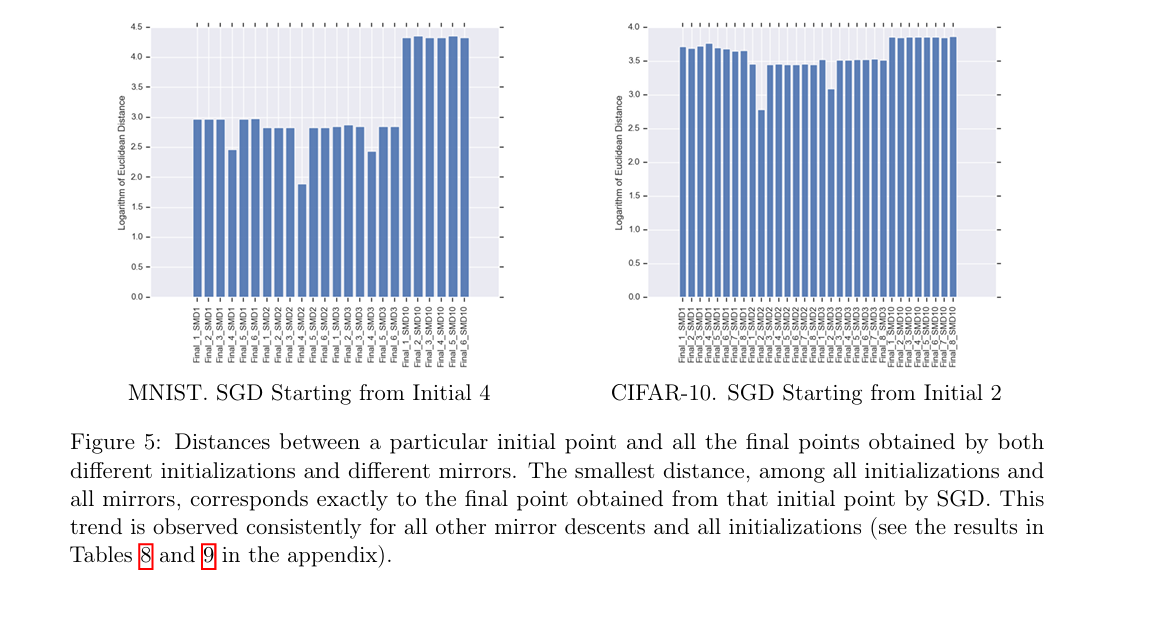
\includegraphics[width=0.95\textwidth]{images/L1vsL10.png}
    
    \vspace{-0.15cm}
    {\small Diagonal pattern holds at scale: ResNet-18, 11M parameters, 8 seeds. Compatible with theory.}
\end{frame}

\begin{frame}{Mirror Effects on Final Weight Distributions}
    \vspace{-0.25cm}
    \centering
    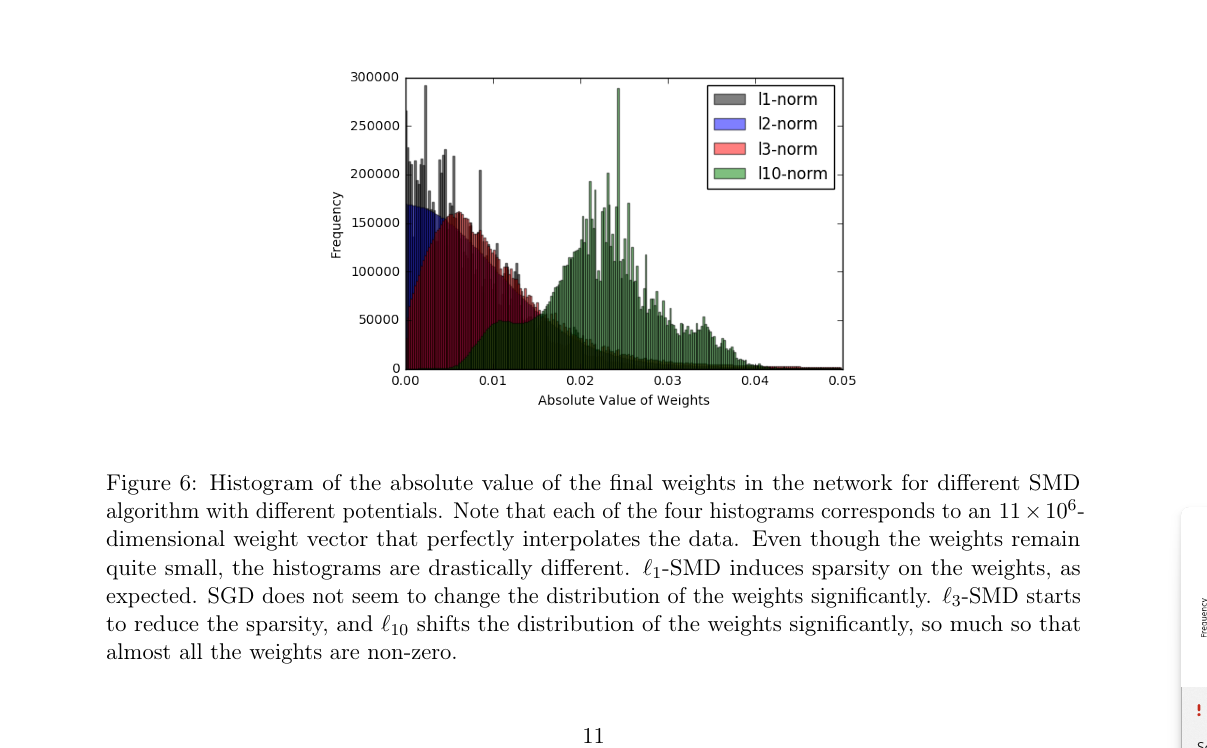
\includegraphics[width=0.92\textwidth]{images/sparsitycomp.png}
    
    \vspace{-0.15cm}
    {\small Mirror choice determines weight magnitude distribution: $\ell_1$ induces sparsity, $\ell_{10}$ creates density.}
\end{frame}

\begin{frame}{Generalization Performance Across Mirrors}
    \vspace{-0.2cm}
    \textbf{MNIST:} All mirrors converge to $\geq 99\%$ test accuracy. Implicit bias does not hurt MNIST generalization.
    
    \vspace{0.15cm}
    \textbf{CIFAR-10:} Mirror choice significantly impacts test error:
    \begin{itemize}
        \item $\ell_{10}$-SMD: Best generalization (densest weights, fewest constraints)
        \item $\ell_2$ (SGD): Intermediate performance
        \item $\ell_3$-SMD: Slightly worse than $\ell_2$
        \item $\ell_1$-SMD: Worst (extreme sparsity overly regularizes)
    \end{itemize}
    
    \vspace{0.15cm}
    \textbf{Insight:} Implicit bias controls generalization. Denser regularization regimes generalize better on complex tasks. Optimizer is a design lever for test performance.
\end{frame}

%%%%%%%%%%%%%%%%%%%%%%%%%%%%%%%%%%%%%%%%
% Section: Conclusion
%%%%%%%%%%%%%%%%%%%%%%%%%%%%%%%%%%%%%%%%
\section{\textbf{\textcolor{purple}{Closing: Summary and Future Work}}}

\subsection{\textbf{\textcolor{purple}{Key Takeaways}}}
\begin{frame}[plain]
    \vfill
    \centering
    \begin{beamercolorbox}[sep=8pt,center,shadow=true,rounded=true]{title}
        \usebeamerfont{title}Summary of Contributions\par%
        \color{oxfordblue}\noindent\rule{10cm}{1pt}
    \end{beamercolorbox}
    \vfill
\end{frame}

\begin{frame}{Summary}
    \vspace{-0.2cm}
    \begin{itemize}
        \item \textbf{Implicit Bias}: Exact characterization in linear case, approximate in nonlinear
        \item \textbf{Star-Convexity}: Local regularity connects linear theory to deep learning
        \item \textbf{Optimizer as Regularizer}: Choice of $\psi$ determines bias and generalization
        \item \textbf{Unified View}: SGD, exponentiated gradient, p-norm algorithms all fit framework
    \end{itemize}
    
    \vspace{0.2cm}
    Generalization is the geometric footprint of the optimizer.
\end{frame}
\subsection{\textbf{\textcolor{purple}{Open Questions and Future Directions}}}

\begin{frame}{Future Work}
    \vspace{-0.2cm}
    \begin{enumerate}
        \item Adaptive optimizers: What is effective $\psi$ for Adam or RMSProp?
        \vspace{0.2cm}
        
        \item Transformer architectures: Does analysis extend to non-Euclidean geometry?
        \vspace{0.2cm}
        
        \item Tighter bounds: Can $o(\epsilon)$ be exact for specific architectures?
        \vspace{0.2cm}
        
        \item Learning $\psi$: Adapt mirror map during training?
    \end{enumerate}
\end{frame}

%%%%%%%%%%%%%%%%%%%%%%%%%%%%%%%%%%%%%%%%
% Section: Question and Answers
%%%%%%%%%%%%%%%%%%%%%%%%%%%%%%%%%%%%%%%%
\section{\textbf{\textcolor{purple}{Question and Answers}}}
\begin{frame}[plain]
    \vfill
    \centering
    \begin{beamercolorbox}[sep=8pt,center,shadow=true,rounded=true]{title}
        \usebeamerfont{title}\insertsectionhead\par%
        \color{oxfordblue}\noindent\rule{10cm}{1pt}
    \end{beamercolorbox}
    \vfill
\end{frame}


\end{document}